\documentclass[a4paper, 12pt]{extarticle}

% Пакеты для поддержки языков
\usepackage[english, russian]{babel}

% Настройка кодировок
\usepackage[T2A]{fontenc}
\usepackage[utf8]{inputenc}

\usepackage[dvipsnames]{xcolor}
\usepackage{listings}
\usepackage{xcolor}

% Настройка отступов от краев страницы
\usepackage[left=3cm, right=1.5cm, top=2cm, bottom=2cm]{geometry}

\usepackage{titleps} % Колонтитулы
\usepackage{subfig} % Для подписей к рисункам и таблицам
\usepackage{graphicx} % Для вставки картинок
\graphicspath{{./img}} % Путь до папки с изображениями

% Пакеты для отрисовки графиков
\usepackage{tikz}
\usetikzlibrary{arrows, positioning, shadows}

\usepackage{stmaryrd} % Стрелки в формулах
\usepackage{indentfirst} % Красная строка после заголовка

% Пакеты для работы с таблицами
\usepackage{hhline} % Улучшенные горизонтальные линии в таблицах
\usepackage{multirow} % Ячейки в несколько строчек в таблицах
\usepackage{longtable} % Многостраничные таблицы
\usepackage{paralist, array} % Список внутри таблицы

\usepackage[normalem]{ulem} % Зачеркнутый текст
\usepackage{upgreek, tipa} % Красивые греческие буквы

% Математические пакеты
\usepackage{amsmath, amsfonts, amssymb, amsthm, mathtools}

\usepackage{nicematrix} % Особые матрицы (Гауссовские)

\definecolor{codegreen}{rgb}{0,0.6,0}
\definecolor{codegray}{rgb}{0.5,0.5,0.5}
\definecolor{codepurple}{rgb}{0.58,0,0.82}
\definecolor{backcolour}{rgb}{0.95,0.95,0.92}

\lstdefinestyle{mystyle}{
	backgroundcolor=\color{backcolour},   
	commentstyle=\color{codegreen},
	keywordstyle=\color{magenta},
	numberstyle=\tiny\color{codegray},
	stringstyle=\color{codepurple},
	basicstyle=\ttfamily\footnotesize,
	breakatwhitespace=false,         
	breaklines=true,                 
	captionpos=b,                    
	keepspaces=true,                 
	numbers=left,                    
	numbersep=5pt,                  
	showspaces=false,                
	showstringspaces=false,
	showtabs=false,                  
	tabsize=2
}

\lstset{style=mystyle}

\linespread{1.5} % Межстрочный интервал
\setlength{\parindent}{1.25cm} % Табуляция
\setlength{\parskip}{0cm}

% Добавляем гипертекстовое оглавление в PDF
\usepackage[
bookmarks=true, colorlinks=true, unicode=true,
urlcolor=black, linkcolor=black, anchorcolor=black,
citecolor=black, menucolor=black, filecolor=black,
]{hyperref}

% Убрать переносы слов
\tolerance=1
\emergencystretch=\maxdimen
\hyphenpenalty=10000
\hbadness=10000

\newpagestyle{main}{
	% Верхний колонтитул
	\setheadrule{0cm} % Размер линии отделяющей колонтитул от страницы
	\sethead{}{}{} % Содержание {слева}{по центру}{справа}
	% Нижний колонтитул
	\setfootrule{0cm} % Размер линии отделяющей колонтитул от страницы
	\setfoot{}{\thepage}{} % Содержание {слева}{по центру}{справа}
}
\pagestyle{main}

% Новые команды
\newcommand{\n}{\par}
\newcommand{\percent}{\mathbin{\%}}

% Заменяем Рис. на Рисунок
\addto\captionsrussian{\renewcommand{\figurename}{Рисунок}}

% Изменение формата подписей
% Стиль номера таблицы/рисунка #1-Таблица/Рисунок. #2-номер
\DeclareCaptionLabelFormat{custom}
{
	#1 #2.
}
% Стиль разделителя номера таблицы/рисунка и названия таблицы/рисунка
\DeclareCaptionLabelSeparator{custom}{}
% Стиль формата #1-номер таблицы/рисунка #2-разделитель #3-название
\DeclareCaptionFormat{custom}
{
	#1 #3
}

\captionsetup
{
	format=custom,
	labelsep=custom,
	labelformat=custom
}

\begin{document}
	\newcommand{\TeacherName}{
		Доцент кафедры высокопроизводительных вычислений и системного программирования,\\ кандидат технических наук:\\ 
		Сысоев А.В.
	}
	\newcommand{\LabName}{Построение выпуклой оболочки для компонент бинарного изображения}
	
	\begin{titlepage}
		\begin{center}
			МИНИСТЕРСТВО НАУКИ И ВЫСШЕГО ОБРАЗОВАНИЯ РОССИЙСКОЙ ФЕДЕРАЦИИ\n
			{\fontsize{14pt}{10pt}\selectfont 
				Федеральное государственное автономное образовательное учреждение высшего образования\n
				\textbf{«Национальный исследовательский Нижегородский государственный университет им. Н.И. Лобачевского»\n
					(ННГУ)}\n
				\vspace{14pt}
				\textbf{Институт информационных технологий, математики и механики}\n
				\vspace{140pt}
				\textbf{ОТЧЁТ ПО ЛАБОРАТОРНОЙ РАБОТЕ}\n
				\vspace{14pt}
				\textbf{«\LabName»}\n
				\vspace{56pt}
			}
		\end{center}
		\hfill
		\begin{minipage}{0.5\textwidth}
			\textbf{Выполнил:\n}
			Студент 3 курса, группы 3821Б1ФИ3:\n
			Володин Евгений Владимирович\n
			
			\textbf{Проверил:\n} 
			\TeacherName\n
		\end{minipage}
		\vfill
		\begin{center}
			Нижний Новгород\n
			2023
		\end{center}
	\end{titlepage}
	\newpage
	\tableofcontents
	\newpage
	\section{Введение}
	В данной лабораторной работе рассматривается задача построения выпуклой оболочки для компонент бинарного изображения. Эта задача относится к области компьютерного зрения, которая занимается анализом изображений и видео с помощью компьютерных алгоритмов. Компьютерное зрение имеет широкое применение в различных сферах, таких как медицина, робототехника, промышленность и безопасность.\n
	Прежде чем перейти к самой лабораторной работе, стоит ввести термины, определяющие её суть.\n
	\textbf{Бинарное изображение} — это изображение, состоящее из двух цветов, обычно черного и белого. Любое бинарное изображение состоит из компонент, количество которых может быть различно.\n
	\textbf{Компонента бинарного изображения} — это связная область одного цвета, например, белая фигура на черном фоне. Чтобы мы могли работать с конкретной компонентой бинарного изображения, их (компоненты) необходимо отличать друг от друга. За это отвечает маркировка связных компонент бинарного изображения, т.е. процесс присвоения уникальных номеров каждой компоненте.\n
	\textbf{Выпуклая оболочка множества точек на плоскости} — это наименьшее выпуклое множество, содержащее все эти точки. Построение выпуклой оболочки для компонент бинарного изображения позволяет выделить их форму и границы, а также получить полезную информацию о их размере, ориентации, количестве и т.д.
	\newpage
	\section{Постановка задачи}
	\textbf{Целью} данной работы является исследование алгоритма построения минимальной выпуклой оболочки для компонент бинарного изображения с использованием последовательного и параллельного подходов, а также сравнение этих двух подходов. Для достижения этой цели необходимо решить следующие \textbf{задачи}:
	\begin{enumerate}
		\item реализовать последовательный алгоритм построения минимальной выпуклой оболочки для компонент бинарного изображения на языке C++;
		\item реализовать параллельный алгоритм построения минимальной выпуклой оболочки для компонент бинарного изображения на языке C++ с использованием технологии MPI;
		\item реализовать ряд тестов с использованием фреймворка Google Test для проверки корректности работы программ;
		\item провести вычислительные эксперименты для сравнения времени работы последовательного и параллельного подходов на разных входных данных и разном числе процессов;
		\item сделать выводы об эффективности и качестве каждого подхода.
	\end{enumerate}
	\newpage
	\section{Описание алгоритма}
	Весь процесс построения выпуклой оболочки для компонент бинарного изображения можно разделить на \textbf{2 этапа}:
	\begin{enumerate}
		\item выделение компонент бинарного изображения;
		\item построение выпуклой оболочки.
	\end{enumerate}
	\subsection{Выделение компонент бинарного изображения}
	На данном этапе каждому пикселю каждой компоненты присваивается номер. Тем самым происходит идентификация каждой компоненты, то есть отделение их друг от друга.\n
	В данной лабораторной работе процесс выделения компонент реализован с помощью циклического алгоритма, использующего очередь задач.
	\subsection{Построение выпуклой оболочки}
	После завершения первого этапа образуется набор компонент. Однако изображение чаще всего имеет достаточно плотную структуру, поэтому в целях оптимизации компоненты дополнительно приводятся к более простому виду. Из рассмотрения удаляются точки, которые имеют более двух ненулевых соседей, а также те, которые имеют двух ненулевых соседей на одной линии (справа и слева или сверху и снизу от текущего пикселя). Данная процедура позволяет уменьшить количество рассматриваемых точек до минимума.\n
	Для построения выпуклой оболочки для каждой компоненты бинарного изображения был выбран алгоритма Грэхема. На вход данному алгоритму подается массив точек, которые принадлежат конкретной компоненте.\n
	Работу данного алгоритма можно разделить на несколько \textbf{этапов}:
	\begin{enumerate}
		\item выбираем точку из массива с минимальной $x$-координатой (если таких несколько, берем самую верхнюю из них), добавляем ее в ответ;
		\item упорядочиваем оставшиеся точки по углу, который они образуют с выбранной точкой;
		\item добавляем в ответ $p_1$ - первую точку из упорядоченного списка;
		\item берем следующую точку $k$, и пока $k$ и две предыдущие точки в текущей оболочке ($p_i$ и $p_{i-1}$) образуют векторы ($p_i$$k$ и $p_i$$p_{i-1}$), которые лежат не по часовой стрелке, исключаем из оболочки $p_i$;
		\item добавляем в оболочку точку $k$;
		\item повторяем пункты 4-5, пока есть точки.
	\end{enumerate}
	\begin{figure}[h]
		\centering
		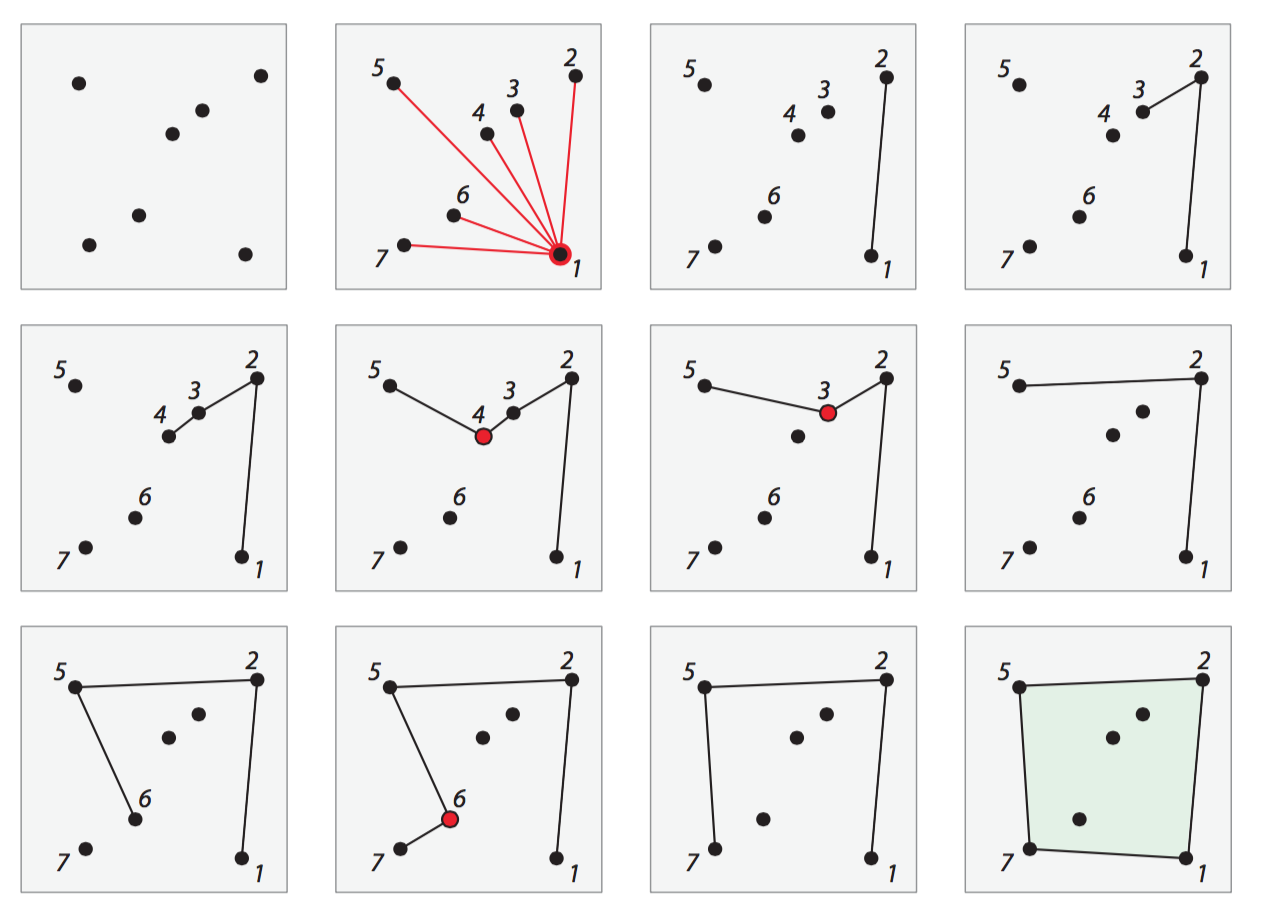
\includegraphics[width=\linewidth]{img/graham}
		\caption{Алгоритм Грэхема в действии. Красные точки образуют левый поворот и удаляются из оболочки.}
		\label{fig:graham}
	\end{figure}
	\newpage
	\section{Описание схемы распараллеливания}
	В последовательной версии алгоритма второй этап происходит независимо для каждой компоненты. Это замечание можно использовать при реализации параллельной версии алгоритма.\n
	Таким образом, каждый процесс получает свою часть компонент (равномерно распределенных), для которых он находит точки, составляющие выпуклые оболочки. Затем результаты, полученные в каждом процессе, отправляются в нулевой процесс, где они собираются в один массив, содержащий координаты точек выпуклых оболочек для каждой компоненты.
	\newpage
	\section{Программная реализация}
	Программа состоит из заголовочного файла $chbi.h$ и двух исходных файлов $chbi.cpp$ и $main.cpp$.\n
	В заголовочном файле определены функции, реализующие последовательный и параллельный подходы для нахождения выпуклой оболочки произвольного множества точек, а также вспомогательные функции: для выделения компонент изображения, для подсчета количества компонент, для сокращения числа точек, генерации примеров и другие.
	
	\subsection{Функции для выделения компонент изображения}
	\begin{lstlisting}[language=C++]
		std::vector<int> findComponents(const std::vector<std::vector<int>>& image, int width, int height);
	\end{lstlisting}
	Функция $findComponents$ является не более чем общим интерфейсом. Она принимает на вход исходное изображение в виде двумерного вектора, его высоту и ширину. Весь процесс выполнения данной функции связан с вызовом для каждого пикселя процедуры $floodFill$. На выходе функция $findComponents$ возвращает промаркированное изображение в виде вектора.
	\begin{lstlisting}[language=C++]
		void floodFill(std::vector<int>* image, int height, int width, int yStart, int xStart, int label);
	\end{lstlisting}
	Процедура $floodFill$ выполняет основную работу, а именно принимает на вход изображение в виде указателя на вектор, его высоту и ширину, точку старта, с которой необходимо начать маркировку и метку, которая присваивается данной компоненте. Данная функция ничего не возвращает, так как изменяет изображение, переданное ей в качестве аргумента.
	
	\subsection{Функции подсчета}
	\begin{lstlisting}[language=C++]
		int findCountComponents(const std::vector<int> &image);
	\end{lstlisting}
	Функция $findCountComponents$ используется для подсчета числа компонент в изображении. На вход принимается изображение в виде ссылки на вектор, а на выходе выдается число компонент в нем. Работает по принципу поиска компоненты с наибольшим номером метки.
	\begin{lstlisting}[language=C++]
		int findCountPointsInComponent(const std::vector<int> &image);
	\end{lstlisting}
	Функция $findCountPointsInComponent$ используется для подсчета числа точек в компоненте. На вход принимается компонента (в виде части изображения), а на выходе выдается число точек в ней. Работает по принципу подсчета ненулевых пикселей.
	
	\subsection{Функция удаления лишний точек компоненты}
	\begin{lstlisting}[language=C++]
		std::vector<int> removeExtraPoints(const std::vector<int> &image, int width, int height, int component);
	\end{lstlisting}
	Функция $removeExtraPoints$ принимает на вход изображение в виде ссылки на вектор, его высоту и ширину, а также номер компоненты, которую необходимо оставить. На выходе получаем изображение в виде вектора, в котором число компонент уменьшено до минимума, что позволяет быстрее строить выпуклую оболочку.
	
	\subsection{Функция алгоритма Грэхема}
	\begin{lstlisting}[language=C++]
		void sort(std::vector<int>* points, int xMin, int yMin);
	\end{lstlisting}
	Функция $sort$ является вспомогательной. Она сортирует точки в процессе работы алгоритма Грэхема. На вход функции подается вектор точек, а также координаты точки, относительно которой нужно выполнить сортировку. На выходе получаем отсортированный по нужному правилу вектор.
	\begin{lstlisting}[language=C++]
		int cross(int x1, int y1, int x2, int y2, int x3, int y3);
	\end{lstlisting}
	Функция $cross$ также является вспомогательной. С помощью нее определяется векторное произведение. На вход подаются координаты точек, а на выходе получаем их векторное произведение.
	\begin{lstlisting}[language=C++]
		std::vector<int> graham(std::vector<int> points);
	\end{lstlisting}
	Функция $graham$ является основной, поскольку реализует алгоритм Грэхема. Она принимает на вход вектор точек. На выходе данная функция возвращает вектор точек, входящих в выпуклую оболочку.
	
	\subsection{Функция, реализующая последовательный подход}
	\begin{lstlisting}[language=C++]
		std::vector<int> getConvexHullSeq(const std::vector<std::vector<int>> &image, int width, int height);
	\end{lstlisting}
	Данная функция принимает на вход изображение в виде ссылки на вектор, его высоту и ширину. В процессе выполнения функции находятся его компоненты, и для каждой из них строится выпуклая оболочка. На выходе получаем вектор точек, которые образуют выпуклые оболочки для каждой компоненты.
	
	\subsection{Функция, реализующая параллельную версию}
	\begin{lstlisting}[language=C++]
		std::vector<int> getConvexHullPar(const std::vector<std::vector<int>> &image, int width, int height);
	\end{lstlisting}
	Данная функция принимает на вход изображение в виде ссылки на вектор, его высоту и ширину. В процессе выполнения функции находятся его компоненты, и для каждой из них строится выпуклая оболочка. На выходе получаем вектор точек, которые образуют выпуклые оболочки для каждой компоненты.
	
	\subsection{Функция заполнения изображения}
	\begin{lstlisting}[language=C++]
	void fillImageRandom(std::vector<std::vector<int>>* image, int width, int height);
	\end{lstlisting}
	Функция $fillImageRandom$ заполняет изображение единицами и нулями. На вход она принимает пустое изображение в виде ссылки на двумерный вектор, его высоту и ширину. Эта функция ничего не возвращает, поскольку изменяет непосредственно принятое изображение.
	\newpage
	\section{Результаты экспериментов}
	Прежде чем приступить к проведению экспериментов я проверил корректность работы последовательного и параллельного алгоритмов. Для этого с помощью фреймворка Google Test мной было разработано 5 тестов, каждый из которых, так или иначе, проверяет работоспособность программы при определенных, изначально заданных условиях. Успешное прохождение всех тестов доказывает корректность работы программы.\n
	Для сравнения производительности последовательной и параллельной версий алгоритма мной были проведены эксперименты на разных размерах входных данных и на разном количестве процессов. При проведении экспериментов использовалась система со следующими \textbf{характеристиками}:
	\begin{itemize}
		\item Процессор: AMD Ryzen 5 4600H, 3.00 ГГц.
		\item Оперативная память: 16 ГБ, DDR4
		\item Операционная система: Windows 10
	\end{itemize}
	По результатам экспериментов был построен график (рис. \ref{fig:results}) зависимости числа точек в изображении от времени, которое тратит та или иная версия алгоритма на его обработку.
	\begin{figure}[h]
		\centering
		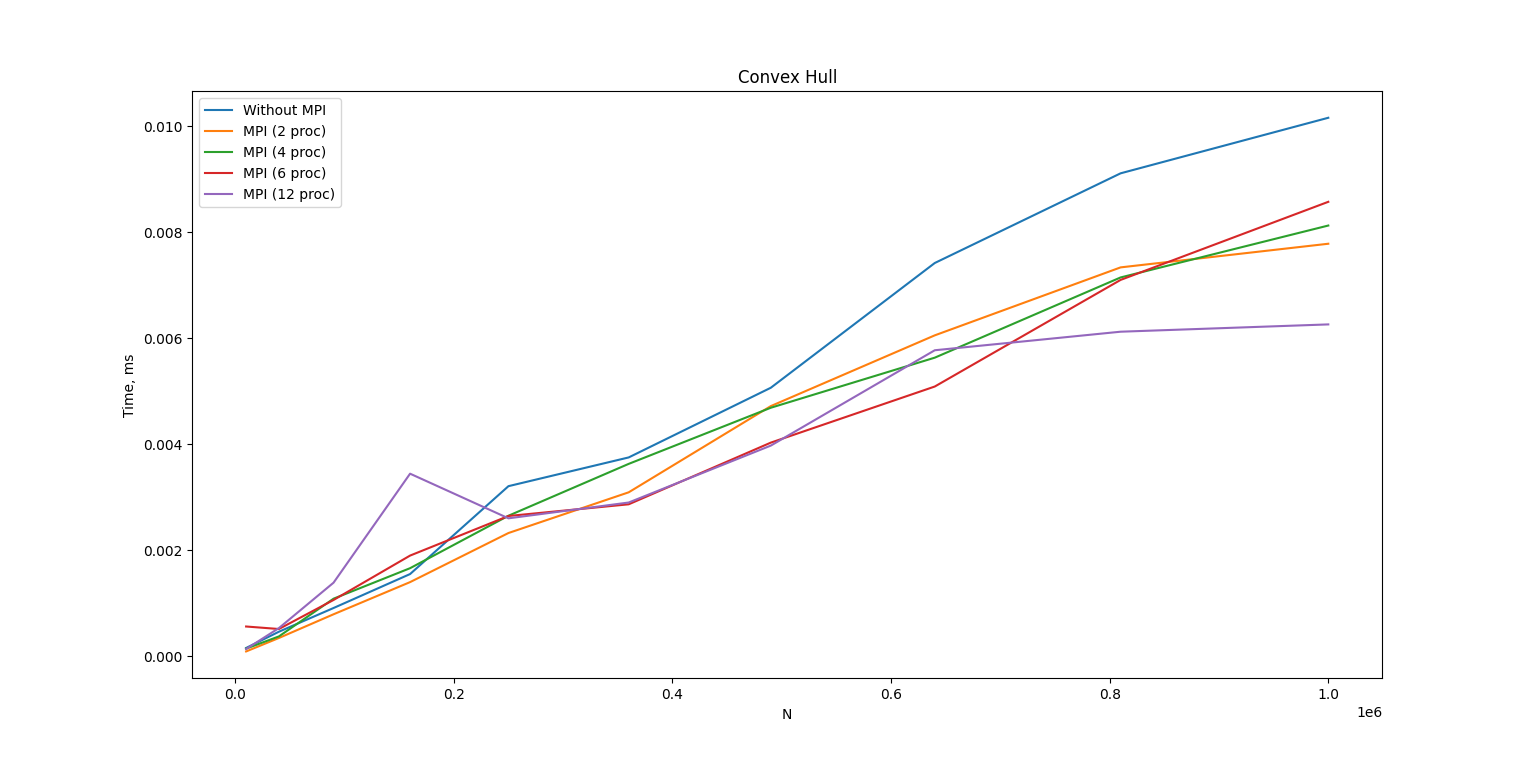
\includegraphics[width=\linewidth]{img/test.png}
		\caption{Результаты экспериментов}
		\label{fig:results}
	\end{figure}
	Также, в ходе эксперимента была сделана выборка нескольких контрольных замеров, результаты которых были сведены в таблицу (табл. \ref{tab:checkpointresults}).
	
	\begin{longtable}[c]{|c|ccccc|}
		\caption{Контрольные значения экспериментов}
		\label{tab:checkpointresults}\\
		\hline
		\multirow{3}{*}{\textbf{\begin{tabular}[c]{@{}c@{}}Количество \\ точек, N\end{tabular}}} & \multicolumn{5}{c|}{\textbf{Время, мс}}                                                                                                                                                                                                                                      \\ \cline{2-6} 
		& \multicolumn{1}{c|}{\multirow{2}{*}{\textbf{\begin{tabular}[c]{@{}c@{}}Без MPI\end{tabular}}}} & \multicolumn{4}{c|}{\textbf{С использованием MPI}}                                                                                                     \\ \cline{3-6} 
		& \multicolumn{1}{c|}{}                                                                                              & \multicolumn{1}{c|}{\textbf{2 процесса}} & \multicolumn{1}{c|}{\textbf{4 процесса}} & \multicolumn{1}{c|}{\textbf{6 процессов}} & \textbf{12 процессов} \\ \hline
		\endfirsthead
		%
		\endhead
		%
		100                                                                                      & \multicolumn{1}{c|}{0.003168}                                                                                      & \multicolumn{1}{c|}{0.119753}            & \multicolumn{1}{c|}{0.157473}            & \multicolumn{1}{c|}{0.18108}              & 0.0737149             \\ \hline
		10000                                                                                    & \multicolumn{1}{c|}{0.16032}                                                                                       & \multicolumn{1}{c|}{0.09476}             & \multicolumn{1}{c|}{0.147707}            & \multicolumn{1}{c|}{0.565167}             & 0.140087              \\ \hline
		90000                                                                                    & \multicolumn{1}{c|}{0.9138324}                                                                                     & \multicolumn{1}{c|}{0.79558}             & \multicolumn{1}{c|}{1.08949}             & \multicolumn{1}{c|}{1.06523}              & 1.39128               \\ \hline
		250000                                                                                   & \multicolumn{1}{c|}{3.210612}                                                                                      & \multicolumn{1}{c|}{2.32737}             & \multicolumn{1}{c|}{2.65317}             & \multicolumn{1}{c|}{2.64831}              & 2.60441               \\ \hline
		490000                                                                                   & \multicolumn{1}{c|}{5.06592}                                                                                       & \multicolumn{1}{c|}{4.71992}             & \multicolumn{1}{c|}{4.68895}             & \multicolumn{1}{c|}{4.0314}               & 3.97537               \\ \hline
		810000                                                                                   & \multicolumn{1}{c|}{9.108408}                                                                                      & \multicolumn{1}{c|}{7.33513}             & \multicolumn{1}{c|}{7.14547}             & \multicolumn{1}{c|}{7.09905}              & 6.12253               \\ \hline
		1000000                                                                                  & \multicolumn{1}{c|}{10.155588}                                                                                     & \multicolumn{1}{c|}{7.78081}             & \multicolumn{1}{c|}{8.12407}             & \multicolumn{1}{c|}{8.57117}              & 6.26017               \\ \hline
	\end{longtable}
	\newpage
	\section{Вывод}
	По графикам, полученным в ходе проведения экспериментов, можно сделать вывод о том, что параллельный алгоритм работает быстрее, чем последовательный.\n
	Да, можно заметить, что при небольшом количестве точек в изображении параллельный алгоритм, особенно если число процессов велико, проигрывает в производительности последовательному, но это происходит потому что большая часть времени уходит на накладные расходы (создание процессов, пересылка данных между ними).\n
	Однако, при росте размера входного изображения и при увеличении числа процессов можно заметить ускорение параллельного алгоритма относительно последовательного. Это означает, что чем больше размер исходного набора точек и чем больше число процессов, тем более быстро будет работать параллельный алгоритм относительно последовательного.\n
	К последнему предложению стоит сделать небольшое замечание, касающееся того, что при очень большом числе процессов параллельный алгоритм может потерять свое ускорение, поскольку, как было сказано ранее, увеличиваются накладные расходы. Поэтому к выбору числа процессов тоже нужно подходить осторожно.
	\newpage
	\section{Заключение}
	В данной лабораторной работе мы реализовали алгоритм построения минимальной выпуклой оболочки для компонент бинарного изображения с использованием последовательного и параллельного подходов.\n
	Наша основная цель была создать эффективный параллельный алгоритм, который бы работал быстрее, чем последовательный, при использовании нескольких процессов.\n
	Мы провели ряд тестов, чтобы проверить корректность наших алгоритмов и сравнить их производительность. Тесты показали, что наши алгоритмы правильно вычисляют оболочку для различных входных данных. Кроме того, мы получили положительные результаты вычислительных экспериментов, которые подтверждают, что наш параллельный алгоритм дает значительное ускорение по сравнению с последовательным.\n
	Таким образом, мы успешно выполнили поставленные задачи и достигли желаемого результата.
	\newpage
	\addcontentsline{toc}{section}{Список литературы}
	\begin{thebibliography}{3}
		\bibitem{Straustrup}
		Страуструп Б. Язык программирования C++. 4-е издание. / Б. Страуструп. – М.: «Бином», 2023. – 1216 с. - ISBN 978-5-6045724-6-7.
		\bibitem{Cormen}
		Кормен, Т.Х. Алгоритмы: построение и анализ, 3-е издание. / Т.Х. Кормен, Ч.И. Лейзерсон, К. Штайн, Р.Л. Ривест. – М.: «Вильямс», 2013. – 1328 с. - ISBN 978-5-8459-1794-2.
		\bibitem{OpenMPI}
		Официальный сайт библиотеки интерфейса передачи сообщений OpenMPI. - Режим доступа: https://www.open-mpi.org
	\end{thebibliography}
	\newpage
	\section*{Приложение}
	\addcontentsline{toc}{section}{Приложение}
	\subsection*{chbi.h}
	\addcontentsline{toc}{subsection}{chbi.h}
	\begin{lstlisting}[language=C++]
// Copyright 2023 Volodin Evgeniy
#ifndef TASKS_TASK_3_VOLODIN_E_CONVEX_HULL_BINARY_IMAGE_CHBI_H_
#define TASKS_TASK_3_VOLODIN_E_CONVEX_HULL_BINARY_IMAGE_CHBI_H_
#include <mpi.h>
#include <iostream>
#include <vector>
#include <queue>
#include <algorithm>
#include <utility>
#include <cmath>
#include <string>
#include <map>
#include <functional>
#include <random>

struct point2d {
	int x, y;
	point2d(int x, int y) : x(x), y(y) {}
};

std::vector<int> findComponents(const std::vector<std::vector<int>>& image, int width, int height);
void floodFill(std::vector<int>* image, int height, int width, int yStart, int xStart, int label);
int findCountComponents(const std::vector<int> &image);
int findCountPointsInComponent(const std::vector<int> &image);
std::vector<int> removeExtraPoints(const std::vector<int> &image, int width, int height, int component);
void sort(std::vector<int>* points, int xMin, int yMin);
std::vector<int> graham(std::vector<int> points);
std::vector<int> getConvexHullSeq(const std::vector<std::vector<int>> &image, int width, int height);
std::vector<int> getConvexHullPar(const std::vector<std::vector<int>> &image, int width, int height);
void fillImageRandom(std::vector<std::vector<int>>* image, int width, int height);

#endif  // TASKS_TASK_3_VOLODIN_E_CONVEX_HULL_BINARY_IMAGE_CHBI_H_
	\end{lstlisting}

\subsection*{chbi.cpp}
\addcontentsline{toc}{subsection}{chbi.cpp}
	\begin{lstlisting}[language=C++]
// Copyright 2023 Volodin Evgeniy
#include "task_3/volodin_e_convex_hull_binary_image/chbi.h"
#include <boost/mpi/communicator.hpp>
#include <boost/mpi/collectives.hpp>

void floodFill(std::vector<int>* image, int height, int width, int yStart, int xStart, int label) {
	std::queue<point2d> tasks;
	tasks.push(point2d(xStart, yStart));
	while (!tasks.empty()) {
		int x = tasks.front().x;
		int y = tasks.front().y;
		tasks.pop();
		if (x >= 0 && y >= 0 && y < height && x < width && image->at(y * width + x) == 1) {
			(*image)[y * width + x] = label;
			tasks.push(point2d(x - 1, y - 1));
			tasks.push(point2d(x - 1, y));
			tasks.push(point2d(x - 1, y + 1));
			tasks.push(point2d(x, y + 1));
			tasks.push(point2d(x + 1, y + 1));
			tasks.push(point2d(x + 1, y));
			tasks.push(point2d(x, y - 1));
			tasks.push(point2d(x + 1, y - 1));
		}
	}
}

std::vector<int> findComponents(const std::vector<std::vector<int>>& image, int width, int height) {
	std::vector<int> image_with_components(width * height);
	for (int i = 0; i < height; ++i) {
		for (int j = 0; j < width; ++j) {
			image_with_components[i * width + j] = image[i][j];
		}
	}
	int label = 2;
	for (int i = 0; i < height; ++i) {
		for (int j = 0; j < width; ++j) {
			if (image_with_components[i * width + j] == 1) {
				floodFill(&image_with_components, height, width, i, j, label);
				++label;
			}
		}
	}
	for (int i = 0; i < height; ++i) {
		for (int j = 0; j < width; ++j) {
			if (image_with_components[i * width + j] != 0) {
				image_with_components[i * width + j]--;
			}
		}
	}
	return image_with_components;
}

int findCountComponents(const std::vector<int> &image) {
	int count_components = 0;
	for (int i = 0; i < image.size(); ++i) {
		if (image[i] > count_components) {
			count_components = image[i];
		}
	}
	return count_components;
}

int findCountPointsInComponent(const std::vector<int> &image) {
	int count_points = 0;
	for (int i = 0; i < image.size(); ++i) {
		if (image[i] != 0) {
			count_points++;
		}
	}
	return count_points;
}

std::vector<int> removeExtraPoints(const std::vector<int> &image, int width, int height, int label) {
	std::vector<int> local_image(image);
	for (int i = 0; i < height; ++i) {
		for (int j = 0; j < width; ++j) {
			if (image[i * width + j] == label) {
				if ((j > 0) && (j < width - 1)) {
					if ((i == 0) || (i == height - 1)) {
						if ((image[i * width + j - 1] == label) && (image[i * width + j + 1] == label)) {
							local_image[i * width + j] = 0;
						}
					}
					if ((i > 0) && (i < height - 1)) {
						if (((image[i * width + j - 1] == label) && (image[i * width + j + 1] == label)) ||
						((image[(i + 1) * width + j] == label) && (image[(i - 1) * width + j] == label))) {
							local_image[i * width + j] = 0;
						}
					}
					continue;
				}
				if ((i > 0) && (i < height - 1)) {
					if ((j == 0) || (j == width - 1)) {
						if ((image[(i - 1) * width + j] == label) &&
						(image[(i + 1) * width + j] == label)) {
							local_image[i * width + j] = 0;
						}
					}
					if ((j > 0) && (j < width - 1)) {
						if (((image[i * width + j - 1] == label) && (image[i * width + j + 1] == label)) ||
						((image[(i + 1) * width + j] == label) && (image[(i - 1) * width + j] == label))) {
							local_image[i * width + j] = 0;
						}
					}
				}
			} else {
				local_image[i * width + j] = 0;
			}
		}
	}
	int size = findCountPointsInComponent(local_image);
	std::vector<int> points(size * 2);
	int k = 0;
	for (int i = 0; i < height; ++i) {
		for (int j = 0; j < width; ++j) {
			if (local_image[i * width + j] != 0) {
				points[k] = j;
				k++;
				points[k] = i;
				k++;
			}
		}
	}
	return points;
}

int cross(int x1, int y1, int x2, int y2, int x3, int y3) {
	return ((x2 - x1) * (y3 - y2) - (x3 - x2) * (y2 - y1));
}

void sort(std::vector<int>* points, int xMin, int yMin) {
	int size = points->size() / 2;
	for (int i = 1; i < size; ++i) {
		int j = i;
		while ((j > 0) && (cross(xMin, yMin, (*points)[2 * j - 2],
		(*points)[2 * j - 1], (*points)[2 * j], (*points)[2 * j + 1]) < 0)) {
			int temp = (*points)[2 * j - 2];
			(*points)[2 * j - 2] = (*points)[2 * j];
			(*points)[2 * j] = temp;
			temp = (*points)[2 * j - 1];
			(*points)[2 * j - 1] = (*points)[2 * j + 1];
			(*points)[2 * j + 1] = temp;
			j--;
		}
	}
}

std::vector<int> graham(std::vector<int> points) {
	std::vector<int> result;
	int num_points = points.size() / 2;
	if (num_points > 1) {
		int x_min = points[0];
		int y_min = points[1];
		int min_index = 0;
		for (int i = 2; i < points.size(); i+=2) {
			if (points[i] < x_min || (points[i] == x_min && points[i + 1] < y_min)) {
				x_min = points[i];
				y_min = points[i + 1];
				min_index = i;
			}
		}
		int temp = points[min_index];
		points[min_index] = points[num_points * 2 - 2];
		points[num_points * 2 - 2] = temp;
		temp = points[min_index + 1];
		points[min_index + 1] = points[num_points * 2 - 1];
		points[num_points * 2 - 1] = temp;
		points.pop_back();
		points.pop_back();
		sort(&points, x_min, y_min);
		result.push_back(x_min);
		result.push_back(y_min);
		result.push_back(points[0]);
		result.push_back(points[1]);
		for (int i = 2; i < points.size(); i += 2) {
			int result_size = result.size();
			int x1 = result[result_size - 4];
			int y1 = result[result_size - 3];
			int x2 = result[result_size - 2];
			int y2 = result[result_size - 1];
			int x3 = points[i];
			int y3 = points[i + 1];
			
			int rot = cross(x1, y1, x2, y2, x3, y3);
			if (rot == 0) {
				result[result_size - 2] = x3;
				result[result_size - 1] = y3;
			} else if (rot < 0) {
				while (cross(result[(result.size()) - 4], result[(result.size()) - 3],
				result[(result.size()) - 2], result[(result.size()) - 1], x3, y3) < 0)
				result.pop_back(), result.pop_back();
				result.push_back(x3);
				result.push_back(y3);
			} else {
				result.push_back(x3);
				result.push_back(y3);
			}
		}
	} else {
		result.resize(2);
		result[0] = points[0];
		result[1] = points[1];
	}
	return result;
}

std::vector<int> getConvexHullSeq(const std::vector<std::vector<int>> &image, int width, int height) {
	std::vector<int> convex_hull;
	std::vector<int> local_image = findComponents(image, width, height);
	int count_components = findCountComponents(local_image);
	for (int i = 1; i <= count_components; ++i) {
		std::vector<int> points = removeExtraPoints(local_image, width, height, i);
		std::vector<int> ch = graham(points);
		for (int j = 0; j < ch.size(); ++j) {
			convex_hull.push_back(ch[j]);
		}
		convex_hull.push_back(-1);
	}
	return convex_hull;
}

std::vector<int> getConvexHullPar(const std::vector<std::vector<int>> &image, int width, int height) {
	std::vector<int> convex_hull;
	
	boost::mpi::communicator world;
	std::vector<int> local_image(width * height);
	int count_components;
	
	if (world.rank() == 0) {
		local_image = findComponents(image, width, height);
		count_components = findCountComponents(local_image);
		for (int i = 1; i < world.size(); ++i) {
			world.send(i, 0, &count_components, 1);
		}
	} else {
		world.recv(0, 0, &count_components, 1);
	}
	
	const int proc_num = std::min(world.size(), count_components);
	if (world.rank() >= proc_num) {
		return std::vector<int>(0);
	}
	
	std::vector<int> components(count_components);
	for (int i = 0; i < count_components; ++i) {
		components[i] = i + 1;
	}
	
	int chunk = count_components / proc_num;
	int rem = count_components % proc_num;
	if (world.rank() < rem) {
		chunk++;
	}
	
	std::vector<int> local_components(chunk);
	
	if (world.rank() == 0) {
		for (int i = 1; i < proc_num; ++i) {
			world.send(i, 0, local_image.data(), width * height);
		}
	} else {
		world.recv(0, 0, local_image.data(), width * height);
	}
	if (world.rank() != 0) {
		world.send(0, 0, &chunk, 1);
	}
	if (world.rank() == 0) {
		int index = 0;
		for (int i = 1; i < proc_num; ++i) {
			int proc_chunk;
			world.recv(i, 0, &proc_chunk, 1);
			world.send(i, 0, components.data() + index, proc_chunk);
			index += proc_chunk;
		}
		for (int i = index, j = 0; i < count_components; ++i, ++j) {
			local_components[j] = components[i];
		}
	} else {
		world.recv(0, 0, local_components.data(), chunk);
	}
	std::vector<int> local_convex_hull;
	for (int i = 0; i < local_components.size(); ++i) {
		std::vector<int> points = removeExtraPoints(local_image, width, height, local_components[i]);
		std::vector<int> ch = graham(points);
		for (int j = 0; j < ch.size(); ++j) {
			local_convex_hull.push_back(ch[j]);
		}
		local_convex_hull.push_back(-1);
	}
	if (world.rank() == 0) {
		int size = 2 * findCountPointsInComponent(local_image);
		size += findCountComponents(local_image);
		for (int i = 1; i < proc_num; ++i) {
			std::vector<int> buffer(size);
			world.recv(i, 0, buffer.data(), size);
			for (int i = 0; i < size; ++i) {
				if (buffer[i] == -1 && buffer[i+1] == 0) {
					convex_hull.push_back(buffer[i]);
					break;
				}
				convex_hull.push_back(buffer[i]);
			}
		}
		for (int i = 0; i < local_convex_hull.size(); ++i) {
			convex_hull.push_back(local_convex_hull[i]);
		}
	} else {
		world.send(0, 0, local_convex_hull.data(), local_convex_hull.size());
	}
	return convex_hull;
}

void fillImageRandom(std::vector<std::vector<int>>* image, int width, int height) {
	std::default_random_engine rnd;
	std::uniform_int_distribution<> dist(0, 1);
	
	for (int i = 0; i < height; ++i) {
		for (int j = 0; j < width; ++j) {
			int pixel = dist(rnd);
		}
	}
}
\end{lstlisting}

\subsection*{main.cpp}
\addcontentsline{toc}{subsection}{main.cpp}
	\begin{lstlisting}[language=C++]
// Copyright 2023 Volodin Evgeniy
#include <gtest/gtest.h>
#include "task_3/volodin_e_convex_hull_binary_image/chbi.h"
#include <boost/mpi/environment.hpp>
#include <boost/mpi/communicator.hpp>

TEST(Parallel_Operations_MPI, Rectangular_Image) {
	boost::mpi::communicator world;
	const int width = 8, height = 5;
	std::vector<std::vector<int>> image({
		{0, 1, 0, 0, 0, 1, 1, 1},
		{1, 1, 0, 0, 1, 1, 1, 1},
		{1, 1, 0, 1, 1, 1, 1, 1},
		{1, 0, 0, 1, 0, 0, 0, 1},
		{1, 1, 0, 0, 0, 0, 1, 1}
	});
	
	std::vector<int> convex_hull_par = getConvexHullPar(image, width, height);
	
	if (world.rank() == 0) {
		std::vector<int> convex_hull_seq = getConvexHullSeq(image, width, height);
		
		for (int i = 0; i < convex_hull_par.size(); ++i) {
			ASSERT_EQ(convex_hull_par[i], convex_hull_seq[i]);
		}
	}
}

TEST(Parallel_Operations_MPI, Square_Image) {
	boost::mpi::communicator world;
	const int width = 10, height = 10;
	std::vector<std::vector<int>> image = {
		{1, 1, 1, 0, 0, 0, 1, 1, 1, 1},
		{1, 1, 0, 0, 0, 0, 0, 1, 1, 1},
		{1, 0, 0, 0, 0, 0, 0, 0, 1, 1},
		{0, 0, 0, 0, 0, 0, 1, 0, 0, 1},
		{0, 0, 0, 1, 0, 1, 0, 0, 0, 0},
		{0, 0, 0, 0, 1, 1, 0, 0, 0, 0},
		{0, 0, 0, 0, 0, 0, 0, 0, 0, 0},
		{1, 1, 1, 0, 0, 0, 0, 1, 1, 1},
		{1, 1, 1, 0, 0, 0, 1, 1, 1, 1},
		{1, 1, 1, 0, 0, 1, 1, 1, 1, 1},
	};
	
	std::vector<int> convex_hull_par = getConvexHullPar(image, width, height);
	
	if (world.rank() == 0) {
		std::vector<int> convex_hull_seq = getConvexHullSeq(image, width, height);
		
		for (int i = 0; i < convex_hull_par.size(); ++i) {
			ASSERT_EQ(convex_hull_par[i], convex_hull_seq[i]);
		}
	}
}

TEST(Parallel_Operations_MPI, Random_Square_Image) {
	boost::mpi::communicator world;
	const int width = 12, height = 12;
	std::vector<std::vector<int>> image(height, std::vector<int>(width, 0));
	
	if (world.rank() == 0) {
		fillImageRandom(&image, width, height);
	}
	
	std::vector<int> convex_hull_par = getConvexHullPar(image, width, height);
	
	if (world.rank() == 0) {
		std::vector<int> convex_hull_seq = getConvexHullSeq(image, width, height);
		
		for (int i = 0; i < convex_hull_par.size(); ++i) {
			ASSERT_EQ(convex_hull_par[i], convex_hull_seq[i]);
		}
	}
}

TEST(Parallel_Operations_MPI, Random_Rectangular_Image_Small) {
	boost::mpi::communicator world;
	const int width = 7, height = 8;
	std::vector<std::vector<int>> image(height, std::vector<int>(width, 0));
	
	if (world.rank() == 0) {
		fillImageRandom(&image, width, height);
	}
	
	std::vector<int> convex_hull_par = getConvexHullPar(image, width, height);
	
	if (world.rank() == 0) {
		std::vector<int> convex_hull_seq = getConvexHullSeq(image, width, height);
		
		for (int i = 0; i < convex_hull_par.size(); ++i) {
			ASSERT_EQ(convex_hull_par[i], convex_hull_seq[i]);
		}
	}
}

TEST(Parallel_Operations_MPI, Random_Rectangular_Image_Big) {
	boost::mpi::communicator world;
	const int width = 35, height = 20;
	std::vector<std::vector<int>> image(height, std::vector<int>(width, 0));
	
	if (world.rank() == 0) {
		fillImageRandom(&image, width, height);
	}
	
	std::vector<int> convex_hull_par = getConvexHullPar(image, width, height);
	
	if (world.rank() == 0) {
		std::vector<int> convex_hull_seq = getConvexHullSeq(image, width, height);
		
		for (int i = 0; i < convex_hull_par.size(); ++i) {
			ASSERT_EQ(convex_hull_par[i], convex_hull_seq[i]);
		}
	}
}

int main(int argc, char* argv[]) {
	boost::mpi::environment env(argc, argv);
	boost::mpi::communicator world;
	::testing::InitGoogleTest(&argc, argv);
	::testing::TestEventListeners& listeners = ::testing::UnitTest::GetInstance()->listeners();
	if (world.rank() != 0) {
		delete listeners.Release(listeners.default_result_printer());
	}
	RUN_ALL_TESTS();
	return 0;
}
\end{lstlisting}
\end{document}
